\chapter*{\scalebox{5}{\color{black!50}\workplace{About the Author}}}

\begin{wrapfigure}{R}{0cm}
\begin{tikzpicture}[node distance=5mm,
terminal/.style={
% The shape:
rectangle,
minimum size=6mm,
rounded corners=3mm,
% The rest
very thick,
draw=black!50,
top color=white,
bottom color=black!20,
font=\ttfamily}]
\node (foto) [terminal] at (0,0)
{
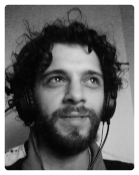
\includegraphics[width=3cm]{./chapters/author.png}
};

\node (rosso) [xshift=-1ex,yshift=1ex] at (foto.south east)
{
\tikz \fill[Indigo] (1ex,1ex) circle (1ex);
};

\node (arancione) at (rosso.center)
{
\tikz \fill[teal] (0.8ex,0.8ex) circle (0.8ex);
};

\node (giallo) at (arancione.center)
{
\tikz \fill[green] (0.6ex,0.6ex) circle (0.6ex);
};

\node (verde) at (giallo.center)
{
\tikz \fill[yellow] (0.4ex,0.4ex) circle (0.4ex);
};

\node (azzurro) at (verde.center)
{
\tikz \fill[orange] (0.2ex,0.2ex) circle (0.2ex);
};

\node (indaco) at (azzurro.center)
{
\tikz \fill[BrickRed] (0.1ex,0.1ex) circle (0.1ex);
};
%\simplewrap{16}{R}{5cm}{5cm}{}{-1pt}{D. Della Cioppa}{fig:author}
\end{tikzpicture}
\end{wrapfigure}

%\textbf{Daniele Della Cioppa} has been an IT Solutions student with \href{https://aclessex.com/about-us/}{ACL Essex}, developing IT skills across a variety of sectors to meet the needs of today’s workplace. He has designed and implemented TCP/IP-based apps in Android, PostgreSQL Databases following the SOLID principles. He is a language expert who runs the podcast \textbf{\emph{\href{https://open.spotify.com/show/05U0mbJEdy1PtqnXOTFHAR}{Speak Napolitano and Survive in Naples}}}. He has five languages under his belt and a lot of incredibly valuable tips to share on how to most effectively learn a language. 
%
%He became a fan of the Spaced Repetition System and of flashcards thanks to Kahei Lee and his incredible \href{https://www.poeticcantonese.com/}{Poetic Cantonese podcast}, where Kahei shares beautiful insights on the Cantonese language, letting the listener learn step by step. He also gained valuable insights from \href{https://coffeebreaklanguages.com/}{Mark Pentleton's podcast} on language learning techniques. Last but not least, \href{https://www.efficacemente.com/}{Andrea Giuliodori}'s book 'Studia meno studia meglio' has been a great resource for him in learning more efficient and effective study habits
%
%In his spare time he's working on independent projects to explore Android Operating systems capabilities, showcasing his best work on \href{https://danieledellacioppa.github.io/}{his webpage}

\textbf{Daniele Della Cioppa}, an IT Solutions student at \href{https://aclessex.com/about-us/}{ACL Essex}, has developed his IT skills at Federico II University before gaining practical work experience in various sectors with \href{https://www.akhter.co.uk/}{Akter}. This has allowed him to meet the demands of today's workplace. Daniele has a strong background in designing and implementing Android apps, utilizing TCP/IP and PostgreSQL databases while following the SOLID principles. Alongside his technical expertise, Daniele is a language enthusiast who hosts the podcast "\textbf{\emph{\href{https://open.spotify.com/show/05U0mbJEdy1PtqnXOTFHAR}{Speak Napolitano and Survive in Naples}}}," where he shares valuable language-learning tips. Fluent in five languages, he became a fan of the Spaced Repetition System and flashcards after listening to Kahei Lee's "\href{https://www.poeticcantonese.com/}{Poetic Cantonese}" podcast and Mark Pentleton's language-learning techniques podcast. Additionally, he has gained insights from Andrea Giuliodori's book "\href{https://www.efficacemente.com/}{Studia meno studia meglio}," which helped him develop more efficient study habits. In his spare time, Daniele works on independent projects to explore the capabilities of the Android Operating System, which he showcases on \href{https://danieledellacioppa.github.io/}{his webpage}.
